\documentclass{amsart}
\usepackage{graphicx}
\graphicspath{{./}}
\usepackage{hyperref}
\usepackage{csvsimple}
\usepackage{longtable}
\usepackage{lscape}
\usepackage{epigraph}
\title{Statistical Inference of Highly Non-Gaussian Categorical Data}
\author{Zulfikar Moinuddin Ahmed}
\date{\today}
\begin{document}
\maketitle

\section{Introduction}

We have introduced exact inference for certain Barndorff-Nielsen Generalised Hyperbolic Distributions on ordered categorical data from World Values Survey (Wave 7).  

We have set up some statistical inference techniques for Generalised Hyperbolic fit to categorical data.  Recall that inference primarily involves being able to gain some quantitative control over $|x_{est} - x_{true}|$ in probability where $x_{true}$ is the totally unknown Nature's secret of true value of some variable.

\section{Q44 Fit}

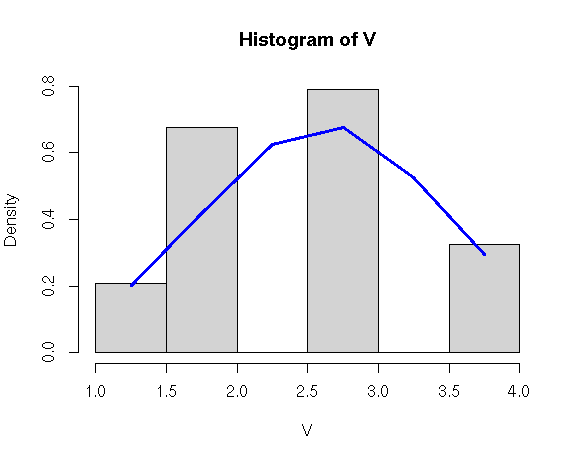
\includegraphics[scale=0.7]{ghdQ44.png}

We want to emphasise here the wonderous issue that the data are not Gaussian and yet there is a beautiful tight fit of GHD.  

\section{Confidence Interval for location Parameter}

\begin{verbatim}
> summary(gg$fit)
Asymmetric Generalized Hyperbolic Distribution:

Parameters:
       lambda     alpha.bar            mu         sigma 
-2.379085e+01  1.264944e+07  2.394619e+00  8.758043e-01 
        gamma 
 2.213342e-01 

Call:
fit.ghypuv(data = x, mu = 0.1, sigma = sd(x), control = list(maxit = 5000))

Optimization information:
log-Likelihood:                -89903.07 
AIC:                           179816.1 
Fitted parameters:             lambda, alpha.bar, mu, sigma, gamma;  (Number: 5)
Number of iterations:          332 
Converged:                     TRUE 
\end{verbatim}

The fit looks good.  Now what is the interval for location parameter $\mu$?

\begin{verbatim}
> gg
$estimate
[1] 2.394619

$low
[1] 2.388619

$high
[1] 2.400619

> gg$high-gg$low
[1] 0.012
\end{verbatim}

The fit is just remarkable, and the true value is not one of the grid point with confidence interval of length 0.012 which is just amazing.

\section{Putting the Quality of this Discovery in Context}

The entire development of probability theory from games of chance in mathematics only slowly led to solution of statistical inference of natural measurements only in 1810 or so.  It was Adrien Marie Legendre who published first on least squares, and it was the development of precise measurements of astronomy and combinations of observations for robust estimates of true value.  From 1810 to 2021 there has never been a single work that I know of that could produce a rigorous theory of statistical inference of continuous distributions that fit natural categorical data.  Now I have shown many beautiful fits of Generalised Hyperbolic distributions to World Values Survey data before, but now we have statistical inference with confidence intervals for location parameters.  I am just delighted by this development, because there is something quite magical about the development of statistical inference with exact models and I have deep conviction regarding how important Ole Barndorff-Nielsen's GHD are universal noise in nature including social science.  This fit is good because it is four-valued.  For two-valued distributions not much will occur but already for four, we can produce robust fits.

\section{Case of Q48}

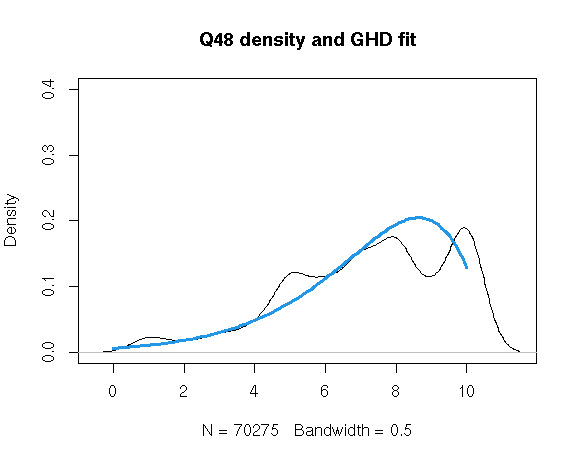
\includegraphics[scale=0.8]{ghdq48.png}

This example of Q48 is too beautiful for words because it is extremely skewed and categorical.  GHD fitting produces extraordinarily good fit.  Location parameter is in the confidence interval 
\[
I = (10.93619,10.96019) )
\]
The width is less than 0.03, and the fit is good.  Inference of this quality for this sort of 'exotic' data is magically good.  Yes these are completely outside the range of all past scientific experience.  The discovery of Ole Barndorff-Nielsen of these GHD models is one of the greatest triumphs of history of science, for while his focus was on distributions of grains of sand, the power of these distributions in Social Science data is beyond all words.


\end{document}